\documentclass[11pt]{beamer}

%\usetheme{Copenhagen}
%\usetheme{Warsaw}
%\usetheme{Frankfurt}
%\usetheme{Darmstadt}
%\usetheme{Berlin}
\usetheme{AnnArbor}
\usefonttheme[onlylarge]{structurebold} 
\setbeamerfont*{frametitle}{size=\normalsize,series=\bfseries} 
\setbeamertemplate{bibliography item}[text]
\setbeamertemplate{navigation symbols}{} 
\usepackage[english]{babel} 
\usepackage[latin1]{inputenc} 
\usepackage{times} 
\usepackage[T1]{fontenc}

\usepackage{tikz} 
\usetikzlibrary{arrows} 
\tikzstyle{block}=[draw opacity=0.7,line width=1.4cm]

\usepackage{ltlfonts}

\usepackage{color} 
\usepackage{alltt} 
\newcommand{\hlstd}[1]{\textcolor[rgb]{0,0,0}{#1}} 
\newcommand{\hlnum}[1]{\textcolor[rgb]{0,0,0}{#1}} 
\newcommand{\hlesc}[1]{\textcolor[rgb]{0,0,1}{#1}} 
\newcommand{\hlstr}[1]{\textcolor[rgb]{0,0,1}{#1}} 
\newcommand{\hldstr}[1]{\textcolor[rgb]{0.5,0.62,0.75}{#1}} 
\newcommand{\hlslc}[1]{\textcolor[rgb]{0.18,0.6,0.34}{#1}} 
\newcommand{\hlcom}[1]{\textcolor[rgb]{0.44,0.48,0.7}{#1}} 
\newcommand{\hldir}[1]{\textcolor[rgb]{0.25,0.37,0.75}{#1}} 
\newcommand{\hlsym}[1]{\textcolor[rgb]{0,0,0}{#1}} 
\newcommand{\hlsymb}[1]{\textcolor[rgb]{1.0,0,0}{#1}} 
\newcommand{\hlline}[1]{\textcolor[rgb]{0,0,0}{#1}} 
\newcommand{\hlkwa}[1]{\textcolor[rgb]{0.5,0,0.33}{\bf{#1}}} 
\newcommand{\hlkwb}[1]{\textcolor[rgb]{0.5,0,0.33}{\bf{#1}}} 
\newcommand{\hlkwc}[1]{\textcolor[rgb]{0.5,0,0.33}{\bf{#1}}} 
\newcommand{\hlkwd}[1]{\textcolor[rgb]{0,0,0}{#1}} 
\definecolor{bgcolor}{rgb}{1,1,1}

\title{Supporting Multi-View Models of Software Systems: Synthesis Techniques} 
\author{Lambeau Bernard} 
\institute{UCL/EPL/INGI} 
\date{dec 2009}

\begin{document}
	\begin{frame}
	    \titlepage 
	\end{frame}

	\begin{frame}{Outline}
		\small
		\tableofcontents
	\end{frame} 

\section{Introduction} 
\begin{frame}{Introduction} 
  \begin{block}{Why Modeling Software Systems?}
    \begin{itemize}
      \item Elaborating requirements and exploring system design \cite{AVL09}
      \item Reasoning about, verifying and documenting systems
    \end{itemize}
  \end{block}
  \begin{block}{Why Multi-View Models?}
    \begin{itemize}
      \item Different models => different but complementary focusses
      \item Example based or rule based? 
      \item Agent interactions or agent internals?
      \item Declarative or operational? 
    \end{itemize}
  \end{block}
  \begin{block}{How Modeling with Multi-View Models?}
    \begin{itemize}
      \item Multi-view framework => inter-model consistency rules
      \item Opportunity for synthesis-driven system modeling 
    \end{itemize}
  \end{block}
\end{frame}

\begin{frame}{Multi-View Models: Golden Triangle} 
    \begin{block}{Scenarios} 
      Typical examples or counterexamples of system behavior through sequences of interactions among agents
      \begin{itemize} \item Example-based, interactions, operational \end{itemize}
    \end{block}
    \begin{block}{Goals} 
      Prescriptive statements of intent whose satisfaction requires cooperation among the agents forming the system
      \begin{itemize} \item Rule-based, interactions as well as agent internals, declarative \end{itemize}
    \end{block}
    \begin{block}{State machines} 
      Classes of required agent behaviors in terms of states and events firing transitions
      \begin{itemize} \item  Rule-based, agent internals, operational \end{itemize}
    \end{block}
\end{frame}

\begin{frame}{Example of synthesis-driven modeling} 
  \begin{center}
    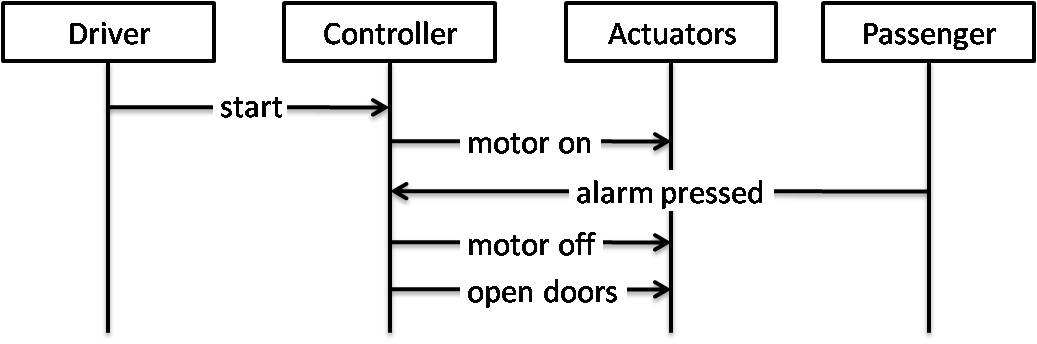
\includegraphics[width=10cm]{train_scenario.jpg}
  \end{center}
  \begin{block}{Synthesize Controller's state machine}
    \begin{itemize}
      \item Accepting at least the sequence of events shown in the example
      \item Under the control of descriptive properties: train doors are either opened or closed but not both in the same state
      \item Under the control of prescriptive properties: train doors must stay closed when the train moves
    \end{itemize}
  \end{block}
\end{frame}

\section{Background}
\subsection{Multi-View Formal Framework}
\begin{frame}{Background: Multi-View Formal Framework}
  \begin{block}{Event-based Behavior Models}
    \begin{itemize}
      \item Scenarios as Message Sequence Charts (MSC)
      \item State machines as Labeled Transition Systems (LTS)
    \end{itemize}
  \end{block}
  \begin{block}{State-based abstractions}
    \begin{itemize}
      \item System state through Fluents
      \item Guards in behavior models (g-LTS and g-hMSC)
      \item Decorations on behavior models
    \end{itemize}
  \end{block}
  \begin{block}{Goals as intentional models}
    \begin{itemize}
      \item Goals and Fluent Linear Temporal Logic (FLTL)
      \item Linking FLTL and LTS: property and tester automata
    \end{itemize}
  \end{block}
\end{frame}

\subsection{Event-based Behavior Models}
\begin{frame}{Message Sequence Charts:  agent interaction examples}
	\begin{center}
		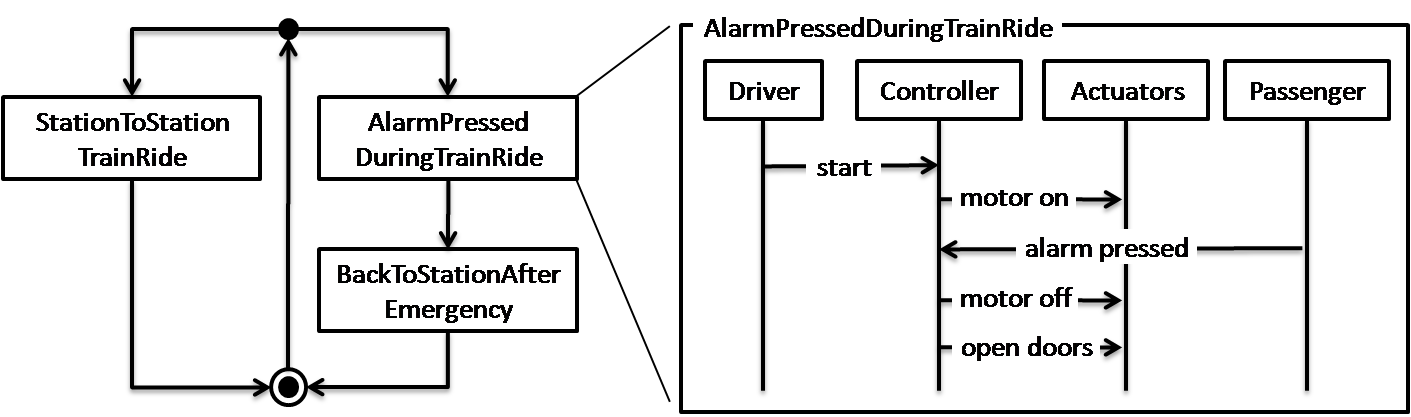
\includegraphics[width=12cm]{Train_hMSC_MSC.png}
	\end{center}
	\begin{block}{MSC (right) and high-level MSC (left)}
		\begin{itemize}
			\item Syntax of MSC and hMSC is described in \cite{ITU96}
			\item Semantics of MSC and hMSC is defined in terms of Labeled Transition Systems, following \cite{Uchitel03}
			\item We also allow a hMSC node to be refined as a finer-grained hMSC
		\end{itemize}
	\end{block}
\end{frame}

\begin{frame}{Labeled Transition Systems (LTS) for agent behaviors}
	\vspace{-0.5cm}
	\begin{center}
		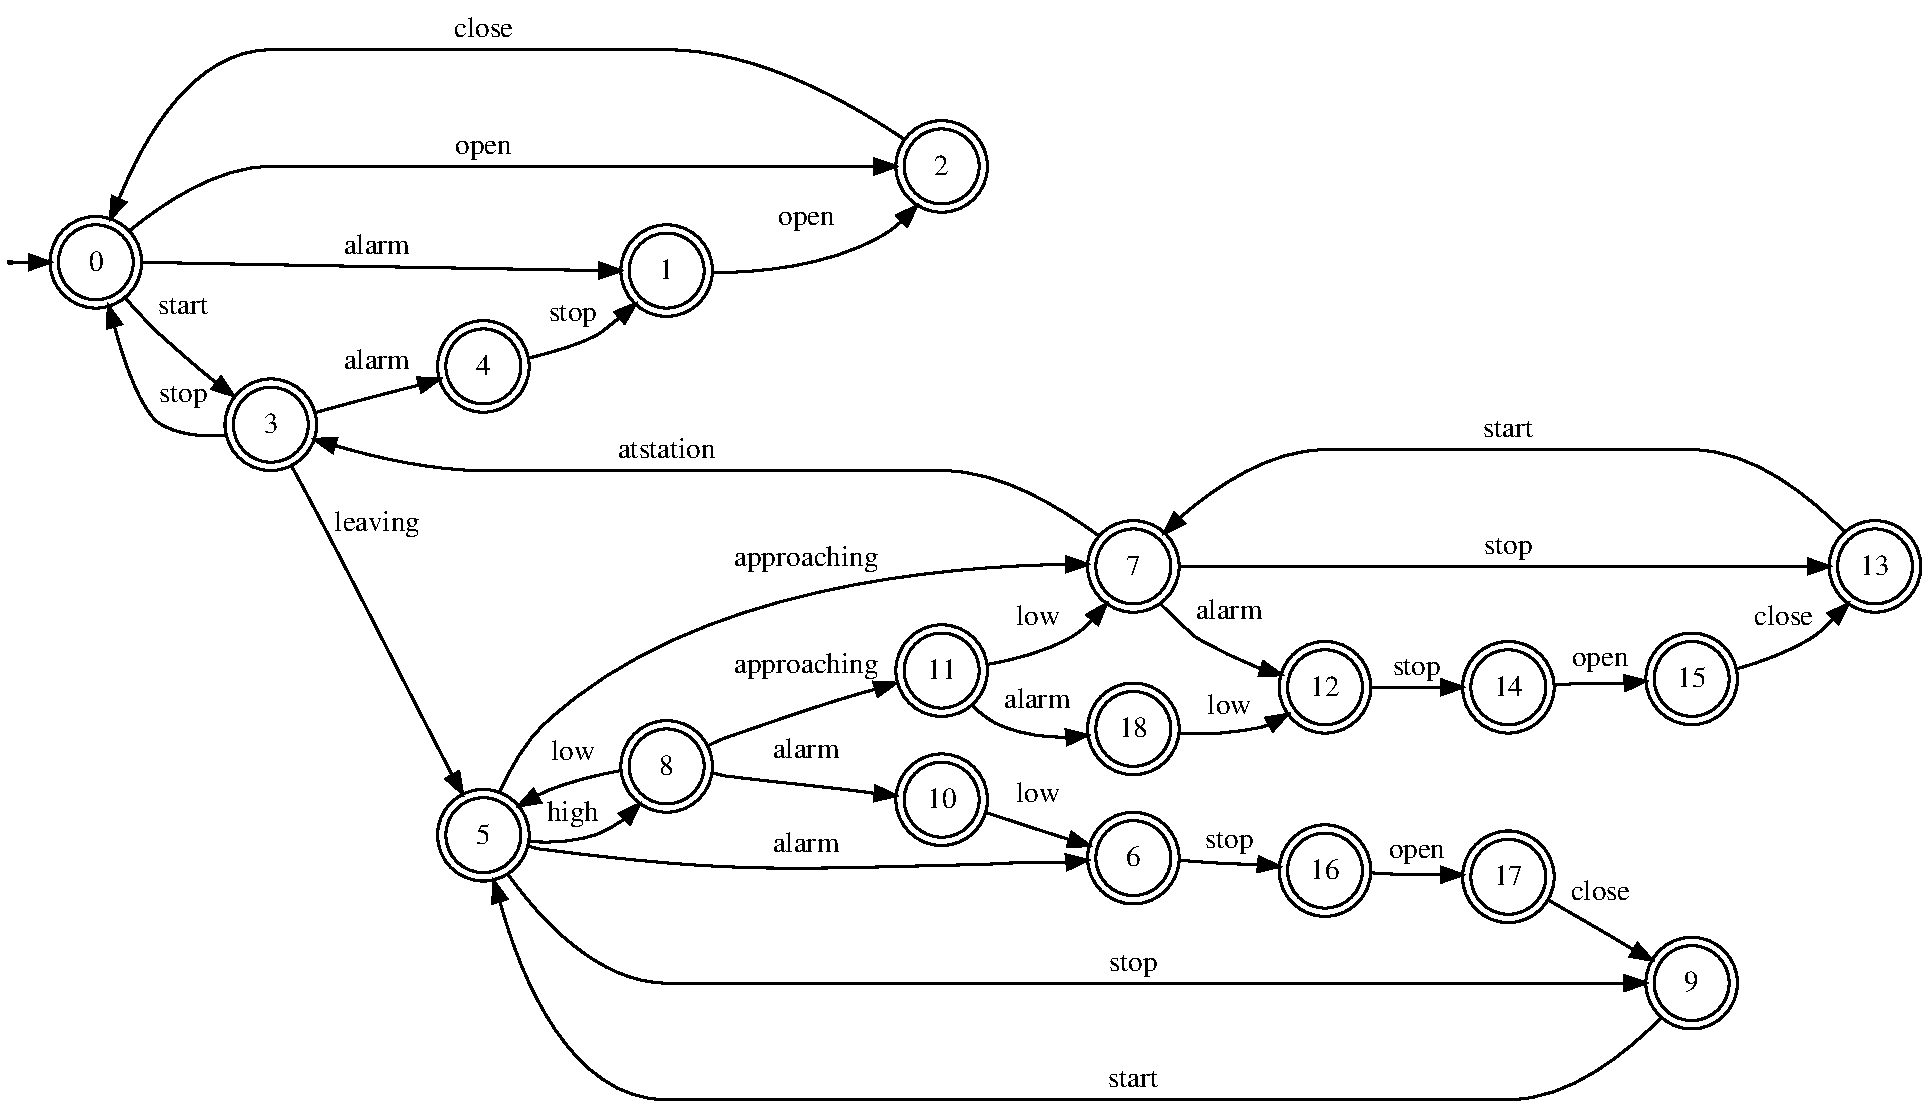
\includegraphics[width=10cm]{bigtrain.pdf}
	\end{center}
	\vspace{-1.5cm}
	\begin{block}{Labeled Transition Systems}
		\begin{itemize}
			\item Syntax and Semantics defined in \cite{Magee99}
			\item Each agent behavior is defined by a LTS. The system behavior is defined by LTS composition \cite{Magee99}
			\item MSCs are admissible traces in the system LTS \cite{Uchitel03}
		\end{itemize}
	\end{block}
\end{frame}

\subsection{State-based abstractions}
\begin{frame}{Capturing state information with Fluents}
	\begin{block}{Fluents capture the system state through the occurrence of events \cite{Milner99}}
		\begin{center}
			$fluent\;Fl = <init_{Fl}, term_{Fl}> initially\;Init_{Fl}$
		\end{center}
		\vspace{-0.4cm}
		where $init_{Fl}$ and $term_{Fl}$ are disjoint set of events rendering the fluent $true$ and $false$, respectively
	\end{block}
	\begin{block}{Example}
		\small
		$fluent\;moving = <start, \{stop, emergency\;stop\}> initially\;false$
		$fluent\;doors\_closed = <close, \{open, emergency\;open\}> initially\;true$
	\end{block}
	\begin{block}{A fluent is ...}
	  	\begin{itemize}
		  	\item ... controlled by an agent if the agent controls (aka emits) all initiating and terminating events of the fluent \cite{Damas06}
			\item ... monitored by an agent if the agent controls or monitors (aka receives) all initiating and terminating events of the fluent
		\end{itemize}
	\end{block}
\end{frame}

\begin{frame}{Guarded Behavior Models}
	\small
	\begin{block}{Summary}
		Guards can be formally used in hMSC and LTS, leading to guarded hMSC (g-hMSC) and guarded LTS (g-LTS)
		\begin{itemize}
		       \item A guard is a boolean expression on fluents
		       \item Structured forms for hMSC and LTS, avoiding state/trace explosion
		       \item Relax the assumption of fluent initial values being known for all instances
		\end{itemize}
	\end{block}
	\begin{block}{Open question, i.e. not discussed in the paper}
		\begin{itemize}
			\item Architectural semantics of guards, i.e. what about guards and agents, guards and LTS composition, guard monitorability
			          and controllability ? 
		\end{itemize}
	\end{block}
	\begin{block}{Related publication}
		\scriptsize
		Damas C., Lambeau B., Roucoux F. and van Lamsweerde A., \emph{Analyzing Critical Process Models through Behavior Model Synthesis},
		in Proc. ICSE'2009: 31th International Conference on Software Engineering, Vancouver, Canada, May 16-24, 2009. 
	\end{block}
\end{frame}

\begin{frame}{Guards in hMSC, i.e. g-hMSC}
	\begin{columns}
		\column{.5\textwidth}
			\begin{block}{Summary}
				\begin{itemize}
					\item \emph{Decision nodes}: outgoing transitions are labeled by boolean expressions on fluents
					\item Initial condition $C_0$ stating an invariant on the initial state
					\item Trace semantics through guarded LTS and LTS
					\item Automated checking of guards: \emph{non overlapping}, \emph{completeness} and \emph{reachability}
				\end{itemize}
			\end{block}
		\column{.5\textwidth}
			\begin{center} 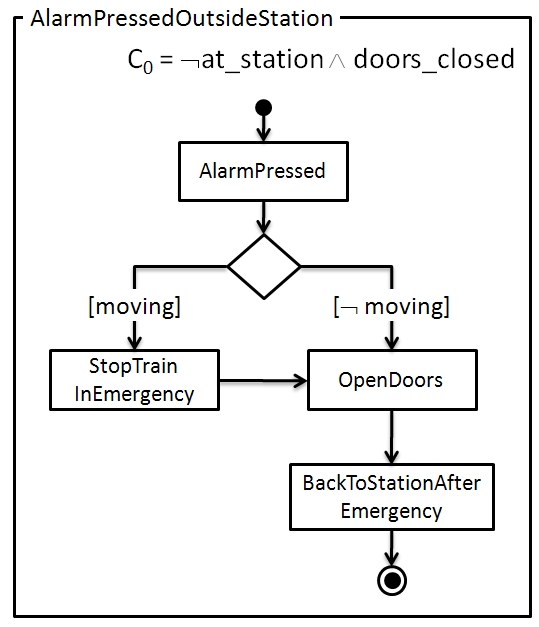
\includegraphics[width=5.5cm]{Train_guarded_hMSC.jpg} \end{center}
	\end{columns}
\end{frame}

\begin{frame}{Guards in LTS, i.e. g-LTS}
	\begin{block}{Summary}
		\begin{itemize}
			\item A g-LTS transition is labeled by an event or a guard
			\item Initial condition $C_0$ stating an invariant on the initial state
			\item A trace is accepted by a g-LTS if three conditions hold: \emph{trace inclusion}, \emph{admissible start} and \emph{guard satisfaction}
		\end{itemize}
	\end{block}
	\begin{block}{Example}
		\begin{center} 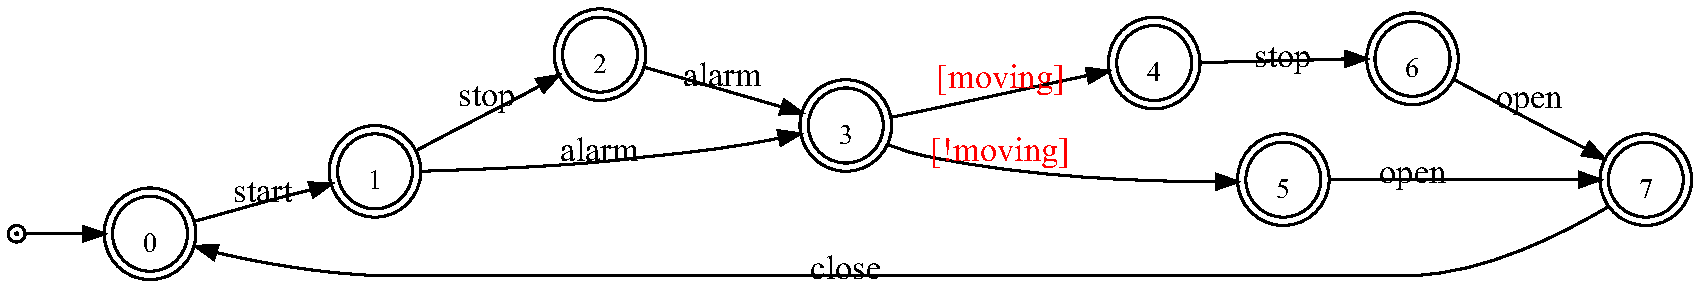
\includegraphics[width=11cm]{Train_guarded_LTS.pdf} \end{center}
		\vspace{-0.5cm}
		\begin{itemize}
			\item $C_0 = \neg moving \wedge doors\_closed$
			\item The event trace $(start\;alarm\;open)$ is not accepted due to the \emph{guard satisfaction} condition
		\end{itemize}
	\end{block}
\end{frame}

\begin{frame}{Decorations on behavior models}
	\begin{block}{Summary}
		\begin{itemize}
			\item \cite{Damas05} proposes a decoration algorithm for generating fluent invariants on LTS states.
			\item In \cite{Damas10} the algorithm is generalized in order to 
				\begin{itemize}
					\item support additional decorations (e.g. cost, doses, time)
					\item support additional transition systems (guarded LTS in particular)
				\end{itemize}
		\end{itemize}
	\end{block}	
	\begin{block}{Example}
		\begin{center} 
			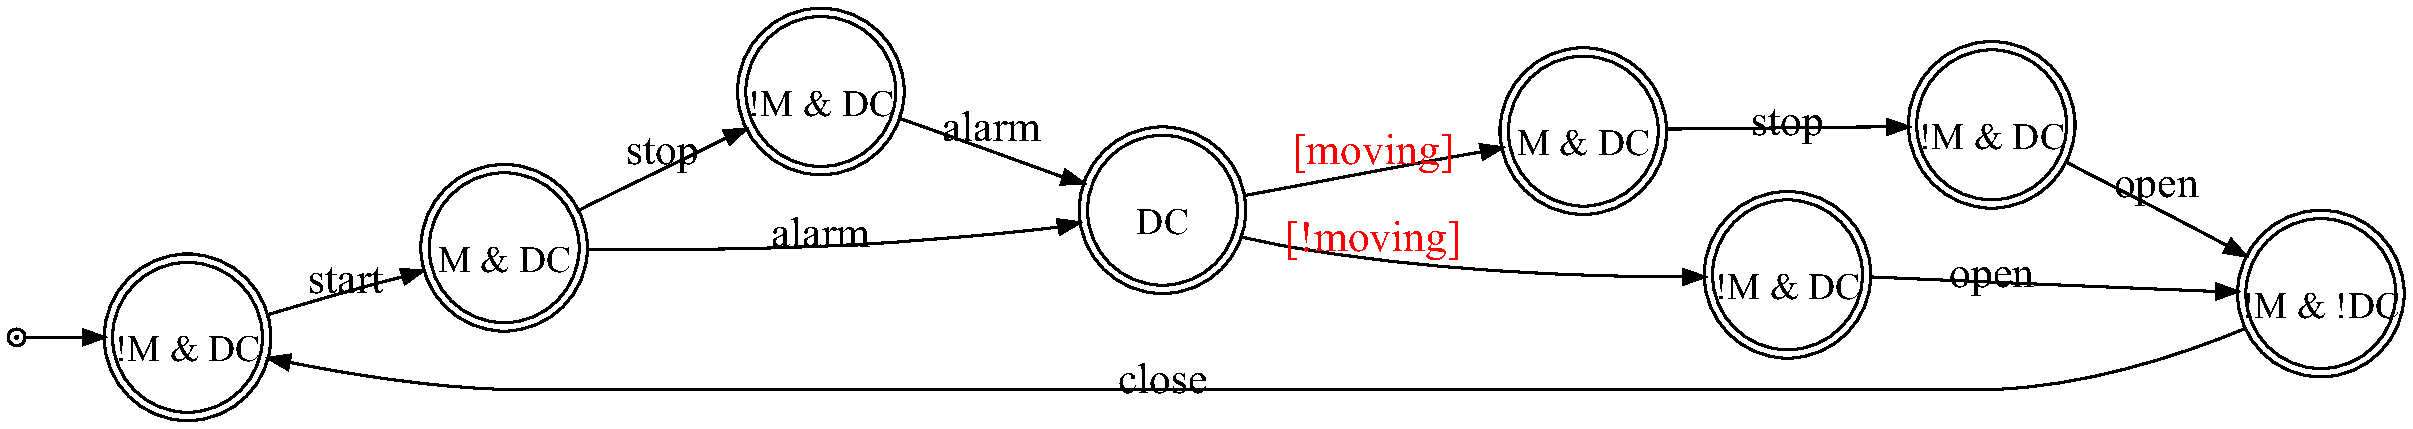
\includegraphics[width=11cm]{Train_guarded_LTS_decorated.pdf}
		\end{center}
		\vspace{-0.5cm}
		\begin{itemize}
			\item where $M$ stands for $moving$ and $DC$ stands for $doors\_closed$
		\end{itemize}
	\end{block}
\end{frame}

\subsection{Goals as intentional models}

\begin{frame}{Goals expressed in FLTL}
	\begin{block}{Goals and Domain properties}
		\begin{itemize}
			\item Goals (resp. Domain properties) are prescriptive properties (resp. descriptive) about the system \cite{AVL09}
			\item Structured in AND/OR graphs
		\end{itemize}
	\end{block}
	\begin{block}{Fluent Linear Temporal Logic (FLTL)}
		\begin{itemize}
			\item Linear Temporal Logic \cite{Manna92} where propositions are Fluents
			\item FLTL is used in \cite{Gianna03} to model-check LTS against (state-based) temporal properties
		\end{itemize}
	\end{block}
	\begin{block}{Example}
		\begin{itemize}
			\item Maintain[DoorsClosedWhileMoving] : Train doors must always remain closed when the train is moving
			\item FormalDef: $\Box(moving \implies doors\_closed) $
		\end{itemize}
	\end{block}
\end{frame}

\begin{frame}{Linking FLTL and LTS}
	\begin{block}{Tester and Property LTS}
		\begin{itemize}
			\item A \emph{Tester LTS} can be synthesized from a FLTL safety property, as explained in \cite{Gianna03}. The error state
			          captures all event traces violating the property
			\item The \emph{Property LTS} obtained by removing the error state captures all event traces not violating the property \cite{Letier08}
		\end{itemize}
	\end{block}
	\begin{block}{Example}
		\vspace{-1cm}
		\begin{columns}
			\column{.5\textwidth}
				\begin{itemize}
					\item $\Box(moving \implies doors\_closed) $
				\end{itemize}
			\column{.5\textwidth}
				\begin{center} 
					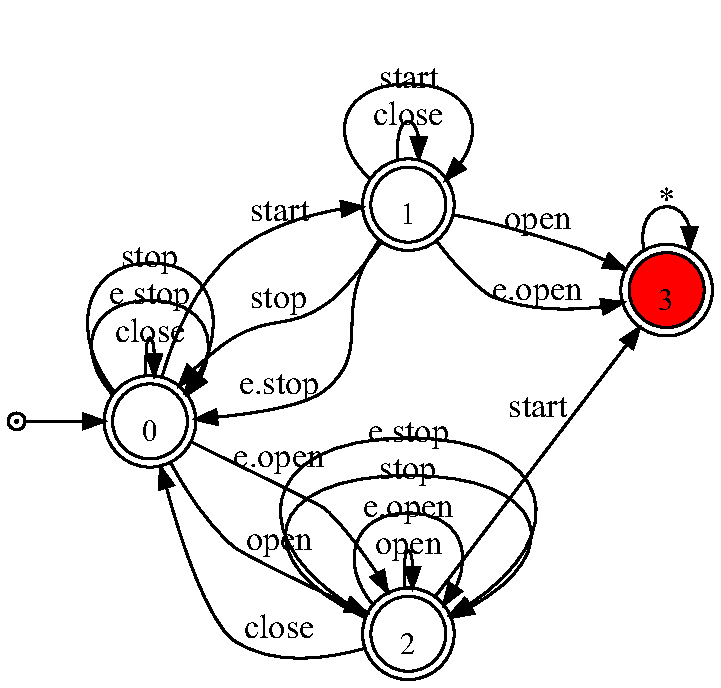
\includegraphics[width=4cm]{MaintainDoorsClosedWhileMoving.pdf}
				\end{center}
		\end{columns}
	\end{block}
\end{frame}

\begin{frame}{Aside: a regular language point of view on Tester and Property LTS}
	\begin{block}{Error state vs. accepting and non accepting states...}
		\begin{itemize}
			\item Property (left) and Tester (right) automata are language complement of each other...
			\item The tester automaton (resp property) accepts all traces violating (resp. not violating) the safety property
		\end{itemize}
	\end{block}
	\begin{block}{Example}
		\vspace{-0.5cm}
		\begin{columns}
			\column{.45\textwidth}
				\begin{center} 
					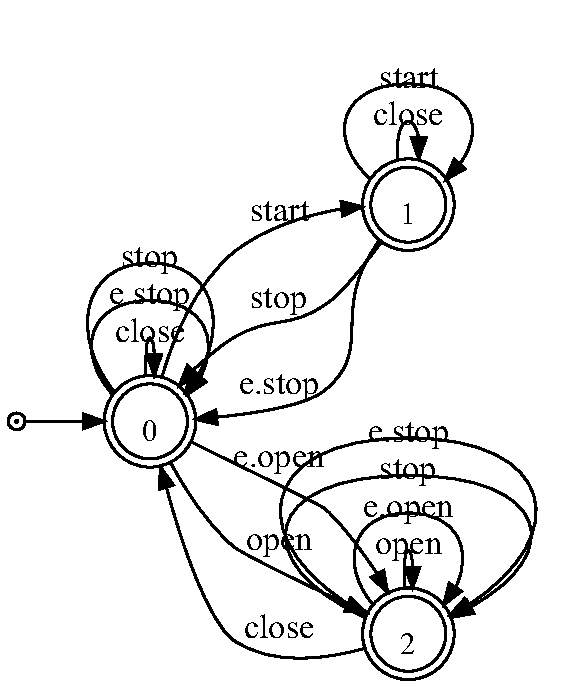
\includegraphics[width=3.5cm, trim=0mm 0mm 0mm 10mm, clip]{MaintainDoorsClosedWhileMoving_property.pdf}
				\end{center}
			\column{.5\textwidth}
				\begin{center} 
					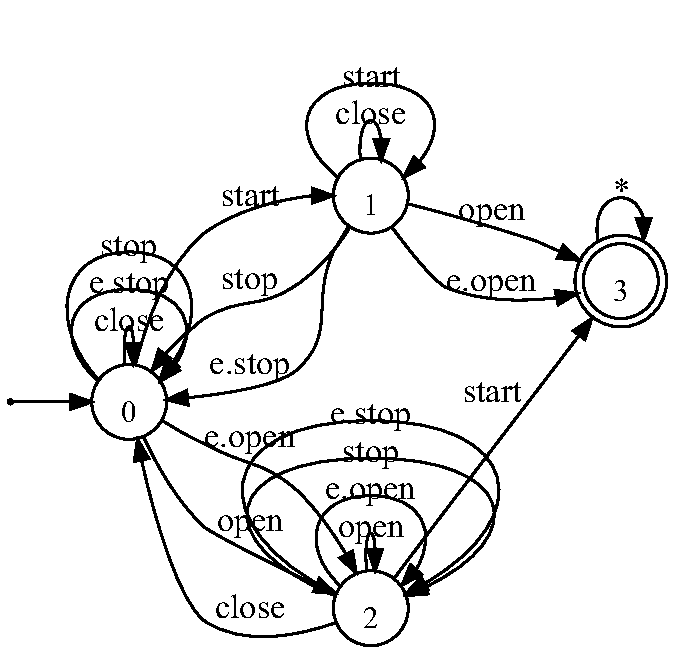
\includegraphics[width=4cm, trim=0mm 0mm 0mm 10mm, clip]{MaintainDoorsClosedWhileMoving_tester.pdf}
				\end{center}
		\end{columns}
	\end{block}
\end{frame}

\section[Deductive Synthesis]{Deductive LTS synthesis from guarded hMSC}
\begin{frame}{Deductive LTS synthesis from guarded hMSC}
	\begin{block}{Question addressed}
		\begin{itemize}
			\item What is the set of event traces accepted by a guarded hMSC?
			\item How to model-check a guarded model?
		\end{itemize}
	\end{block}
	\begin{block}{Main results}
		\begin{itemize}
			\item Adaptation of \cite{Uchitel03} to synthesize a g-LTS from a g-hMSC
			\item LTS composition algorithm for deriving a pure LTS from a g-LTS
			\item Adaptation of \cite{Gianna03} to model-check FLTL properties on g-LTS
		\end{itemize}
	\end{block}
	\begin{block}{Related publications}
	   	\scriptsize
		Damas C., Lambeau B., Roucoux F. and van Lamsweerde A, \emph{Analyzing Critical Process Models through Behavior Model Synthesis},
		in Proc. ICSE'2009: 31th International Conference on Software Engineering, Vancouver, Canada, May 16-24, 2009. 
	\end{block}
\end{frame}

\begin{frame}{Deductive LTS synthesis: what's done, what remains to be done?}
	\begin{block}{Work in progress}
		\begin{itemize}
			\item Full state tracability through the g-hMSC, g-LTS, LTS synthesis (work in progress)
			\item Model-checker feedback in terms of the g-LTS and g-hMSC instead of the pure LTS
		\end{itemize}
	\end{block}
	\begin{block}{Open questions}
		\begin{itemize}
			\item Only applied on the whole system so far, not with different agents in mind (lack of g-LTS composition/decomposition semantics)
		\end{itemize}
	\end{block}
\end{frame}

\section[Inductive Synthesis]{Inductive LTS synthesis from MSC and hMSC}
\begin{frame}{Inductive LTS synthesis from MSC and hMSC}
         \begin{block}{Limitation of deductive approaches}
		\begin{itemize}
			\item Scenarios are known to be inherently partial, they only provide typical examples of system the usage
			\item Therefore, deductive techniques (e.g. \cite{Uchitel03}) can only result in partial LTS
			\item Generalizing observed behaviors looks interesting in practice
		\end{itemize}
	\end{block}
         \begin{block}{About our inductive approach}
		\begin{itemize}
			\item Relies on Grammar Induction (GI), which provides a sound mathematical background
			\item But how to
			\begin{itemize}
				\item Avoid poor behavior generalizations? 
				\item Ensure consistency with other models (state variables, goals, ...)?
				\item Prune the induction process?
			\end{itemize}
		\end{itemize}
	\end{block}
\end{frame}

\subsection{Short background on Grammar Induction}
\begin{frame}{Short background on Grammar Induction}
	\begin{block}{In a few words}
		\begin{itemize}
		 	\item \emph{Grammar induction} aims at learning a regular language $L$ from a set of positive and negative strings,
				 i.e. respectively belonging and not belonging to the language
			\item Also known as \emph{Automaton Induction} when $L$ is represented by a (Deterministic) Finite Automaton $A(L)$
		\end{itemize}
	\end{block}
	\begin{block}{Known results ... among others}
		\begin{itemize}
			\item RPNI algorithm (Regular Positive and Negative Inference)
			\item Necessary condition for convergence: \emph{structural completeness} of the sample (each transition and accepting state 
				of the automaton is used at least once in the input sample)
			\item Sufficient condition for convergence: the input sample contains a \emph{characteristic sample} for $A(L)$
		\end{itemize}
	\end{block}
\end{frame}

\begin{frame}{RPNI algorithm (and variants) in one slide}
	From a Prefix Tree Acceptor, accepting the positive sample only, ...
	\begin{center}
		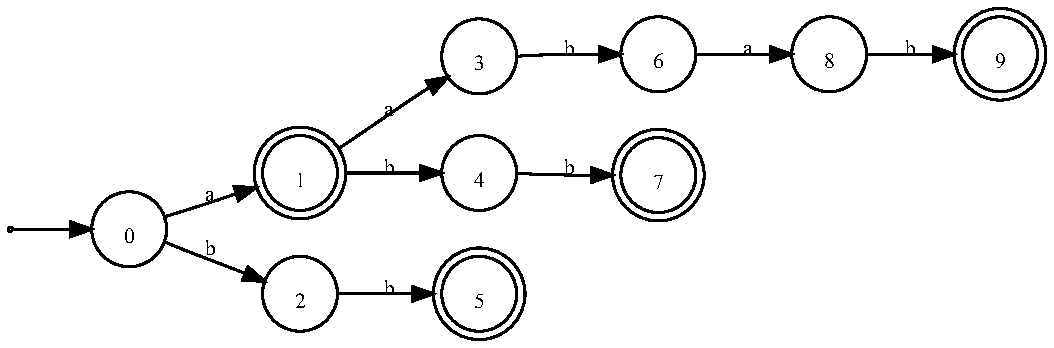
\includegraphics[width=9cm]{dfa_merge_0.pdf}
	\end{center}
	... induce a DFA by successively merging well-chosen state pairs (BlueFringe heuristics), under the control of the negative sample
	\begin{center}
		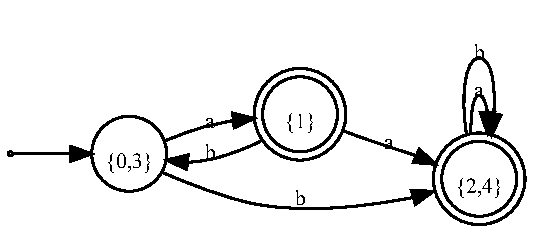
\includegraphics[width=6cm]{dfa_merge_3.pdf}
	\end{center}
\end{frame}

\subsection{Grammar Induction for LTS Synthesis}
\begin{frame}{Grammar Induction for LTS Synthesis ?}
	\begin{block}{Applicability}
		\begin{itemize}
			\item A LTS is a DFA with all accepting states
			\item LTS define a subclass of regular languages (prefix-closed languages)
			\item A positive MSC is an accepting trace in the system LTS (obtained by composition of all agent LTS)
			\item A positive (resp. negative) MSC can be seen as a positive (resp. negative) string of the language accepted by the system LTS
		\end{itemize}
	\end{block}
	\begin{block}{The idea}
		\begin{itemize}
			\item Learn the system LTS from positive and negative scenarios using RPNI
			\item Synthesize agent LTS by projecting the system LTS on their monitored events (standard automaton algorithms)
		\end{itemize}
	\end{block}
\end{frame}

\begin{frame}{Grammar Induction for LTS Synthesis: a short summary}
	\begin{block}{Question addressed}
		\begin{itemize}
			\item Importance of negative strings; are they initially available from end-users?
			\item How to ensure consistency with other models?
			\item Assumption that all MSC start in the same system state, what about loops and reuse?
		\end{itemize}
	\end{block}
	\begin{block}{Main results}
		\begin{itemize}
			\item Our interactive variant of RPNI, namely $QSM$, when few negative scenarios are initially provided
			\item Injecting fluent definitions, goals and legacy components ensures inter-model consistency and prunes the process
			\item Other contributed variants, namely $ASM$ and $ASM^*$, support an hMSC as input, relaxing the assumption mentionned
		\end{itemize}
	\end{block}
\end{frame}

\subsection{Interactive LTS Synthesis from MSC}
\begin{frame}{Interactive LTS Synthesis from MSC: the QSM algorithm}
	\begin{block}{Summary}
		\begin{itemize}
			\item RPNI with BlueFringe heuristic for selecting state pairs to merge
			\item When two states are merged, scenario queries are submitted to an end-user for classification as positive or negative behaviors
			\item The end-user, aka Oracle, guides the induction process, avoiding poor generalizations
			\item Query generation relies on the definition of a \emph{characteristic sample}, which provides a convergence criteria
		\end{itemize}
	\end{block}
	\begin{block}{Related publications}
   		\scriptsize
		\begin{itemize}
			\item Damas C., Lambeau B., and van Lamsweerde A, \emph{Generating Annotated Behavior Models From End-User Scenarios},
			     	IEEE Transactions on Software Engineering, Special Issue on Interaction and State-based Modeling, Vol. 31, No. 12, pp. 1056-1073, 2005.
			\item P. Dupont, B. Lambeau, C. Damas, and A. van Lamsweerde, \emph{The QSM Algorithm and its Application to Software Behavior Model Induction},
         		                   Applied Artificial Intelligence, Vol. 22, 2008, 77-115.
		\end{itemize}
	   \end{block}
\end{frame}

\subsection{Pruning the induction with state decorations}
\begin{frame}{Pruning the induction with fluents}
	\begin{block}{Summary}
		\begin{itemize}
			\item PTA states can be decorated with fluent values, using the decoration algorithm
			\item The induction process can be constrained to avoid merging non equivalent states
		\end{itemize}
	\end{block}
	\begin{center}
		$fluent\;mov(ing) = <start, \{stop, emergency\;stop\}> initially\;false$
	\end{center}
	\begin{center}
		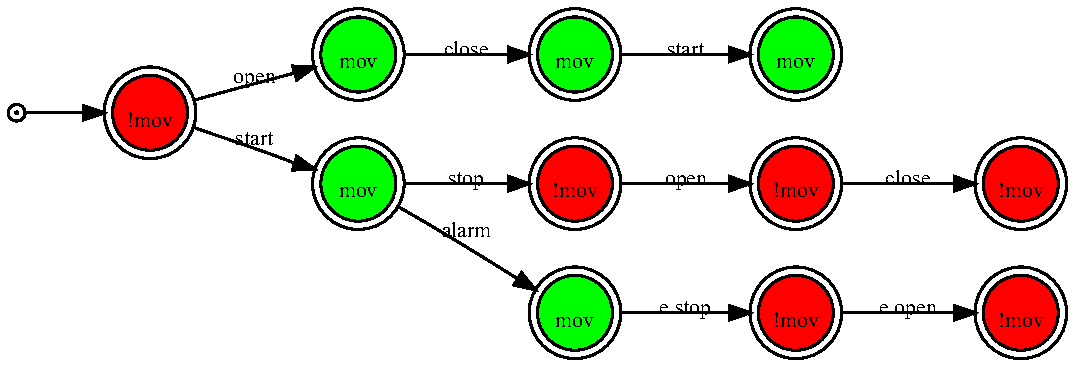
\includegraphics[width=9cm]{train_pta.pdf}
	\end{center}
\end{frame}

\subsection{Pruning the induction with goals}
\begin{frame}{Pruning the induction with goals}
	\begin{block}{Summary}
		\begin{itemize}
			\item Color PTA states with corresponding states in the tester. Avoid merging two PTA states not sharing the color
		\end{itemize}
	\end{block}
	\begin{columns}
		\column{.45\textwidth}
			\begin{center}
				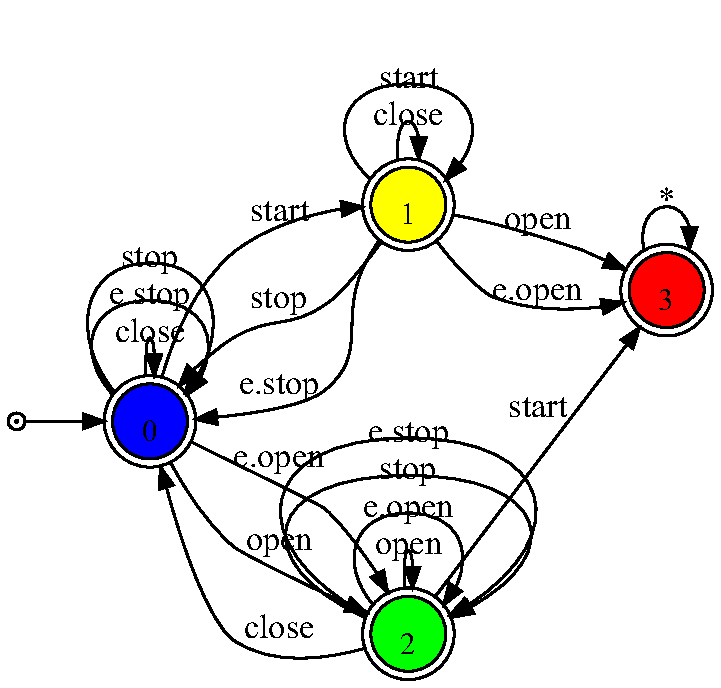
\includegraphics[width=4cm, trim = 0mm 0mm 0mm 10mm, clip]{MaintainDoorsClosedWhileMoving_colored.pdf}
			\end{center}
		\column{.45\textwidth}
			\begin{center}
				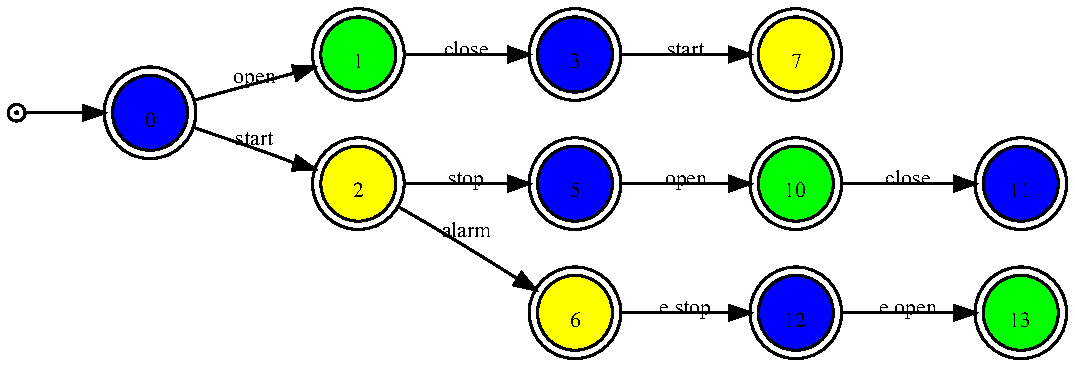
\includegraphics[width=5.5cm, trim = 0mm 0mm 0mm 0mm, clip]{train_pta_decorated.pdf}
			\end{center}
	\end{columns}
	\begin{block}{Open questions}
		\begin{itemize}
			\item Sound but too strong! This is related to another open issue on $ASM^*$ about the negative language $L^-$ (see later)
		\end{itemize}
	\end{block}
\end{frame}

\begin{frame}{Pruning the induction though equivalence classes}
	\begin{block}{State coloring as a generalization}
		\begin{itemize}
			\item Equivalence relations can be defined on PTA states and induction process constrained to avoid merging
				non equivalent states.
			\item Legacy components can be used in a similar way, for example
		\end{itemize}
	\end{block}
	\begin{block}{Open questions}
		\begin{itemize}
			\item Defining equivalence classes could be extended in the light of lattice-based decorations
			\item We are convinced that additional architectural constraints could be used (to avoid introducing implied scenarios, for example)
		\end{itemize}
	\end{block}
	\begin{block}{Related publications}
   		\scriptsize
		\begin{itemize}
			\item C. Damas, B. Lambeau and A. van Lamsweerde, \emph{Scenarios, Goals, and State Machines: a Win-Win Partnership for Model Synthesis}, 
                                      Proc. FSE'06: Intl. ACM Symposium on the Foundations of Software Engineering, Portland (OR), November 2006. 
		\end{itemize}
	   \end{block}
\end{frame}

\subsection{Pruning the induction with control information}
\begin{frame}{Pruning the induction with control information}
	\begin{block}{Questions addressed}
		\begin{itemize}
			\item Assumption that all MSCs start in the same initial state
			\item End-users would like to capture loops when known
			\item Would it be possible to take a hMSC as input instead of a collection of MSCs?
		\end{itemize}
	\end{block}
	\begin{block}{Main results}
		\begin{itemize}
			\item Introduction of \emph{mandatory merge constraints} on PTA states, which is the logical counterpart
				of equivalence classes
			\item The $ASM$ algorithm generalizes a positive language $L^+$ under the control of a negative sample $S^-$. 
			          $ASM^*$ generalizes a positive language $L^+$ under the control of a negative language $L^-$
			\item Therefore, behaviors described in a hMSC can be generalized under the control of negative MSCs 
		\end{itemize}
	\end{block}
\end{frame}

\begin{frame}{Pruning the induction with control information}
	\begin{block}{Open questions}
		\begin{itemize}
			\item Three concurrent techniques about pruning with goals: equivalent classes (too strong), $ASM^*$ (looks not 
				applicable directly) and Coste's work in \cite{Coste04}
			\item $ASM$ and $ASM^*$ do not support the BlueFringe heuristics nor the interactive feature
			\item Theoretical GI questions because $ASM$ and $ASM^*$ do not perfectly fit the classical regular language learning framework
		\end{itemize}
	\end{block}
	\begin{block}{Related publications}
   		\scriptsize
		\begin{itemize}
			\item B. Lambeau, C. Damas and P. Dupont, \emph{State-merging DFA Induction Algorithms with Mandatory Merge Constraints}, 
	                             Lecture Notes in Artificial Intelligence No. 5278, Springer, pp. 139-153, 2008, 9th International Colloquium on Grammatical Inference, 
	                             St Malo, France, September 22-24.
			\item No feedback in the RE community so far
		\end{itemize}
	   \end{block}
\end{frame}

\section{Evaluation and Tool Support}
\begin{frame}{Evaluation}
	\begin{block}{Deductive synthesis evaluation}
		\begin{itemize}
			\item Usage of the g-hMSC model-checker is illustrated on a case study in \cite{Damas09}
			\item Additional case-studies: work in progress 
		\end{itemize}
	\end{block}
	\begin{block}{Inductive synthesis evaluation}
		\begin{itemize}
			\item Number of generated queries and convergence of QSM have been evaluated on RE case studies and synthetic data in \cite{Damas05} and \cite{Dupont08}
			\item Evaluation of the pruning techniques on RE case studies in \cite{Damas06}
			\item Evaluation protocol for $ASM$ in \cite{Lambeau08}, applied on one RE case study and synthetic data
		\end{itemize}
	\end{block}
\end{frame}

\begin{frame}{Tool Support}
	\begin{block}{Induction Toolkit}
		\begin{itemize}
			\item Recent refactoring of all the automaton tools (still in progress)
			\item Light release will be provided during the Stamina induction competition (2010)
			\item Full release will be provided after the competition (few work remaining here)
		\end{itemize}
	\end{block}
	\begin{block}{A FLTL model-checker for g-hMSC models}
		\begin{itemize}
			\item Work in progress (architecture and packaging of the tool support)
			\item Future collaboration with Antoine Cailliau for additional (F)LTL tools (master thesis)
		\end{itemize}
	\end{block}
\end{frame}

\section{Conclusion}
\begin{frame}{Conclusion}
	\begin{block}{My two-cent point-of-view}
		\begin{itemize}
			\item We must further investigate the LTS theory in the light of regular languages (composition, tester and property LTS, \ldots)
			\item The way guards are formally defined in the g-hMSC/g-LTS paper is not really convincing
			\item What about a sound theory about guarded LTS (composition, minimality, \ldots) ?
		\end{itemize}
	\end{block}
\end{frame}

\section{References}

\begin{frame}[allowframebreaks]{References}
	\tiny
	\bibliographystyle{alpha}
	\bibliography{slides} 
\end{frame}

\end{document}